\documentclass[11pt]{article}

% ------------------------------------------------------------
% Standard LaTeX packages
% ------------------------------------------------------------
\usepackage[margin=1in]{geometry}
\usepackage{amsmath,amssymb,mathtools}
\usepackage{amsthm}
\usepackage[american]{babel}
\usepackage{stmaryrd}
\usepackage{enumitem}
\usepackage{booktabs}
\usepackage{array}
\usepackage{listings}
\usepackage[x11names,table]{xcolor}
\usepackage{mdframed}
\usepackage{tikz}
\usetikzlibrary{arrows.meta,positioning,calc,decorations.pathmorphing}
\usepackage{url}
\usepackage[colorlinks=true,linkcolor=blue,citecolor=blue,urlcolor=blue]{hyperref}

% ---------- Theorem environments ----------
\theoremstyle{plain}
\newtheorem{theorem}{Theorem}[section]
\newtheorem{proposition}[theorem]{Proposition}
\newtheorem{lemma}[theorem]{Lemma}
\newtheorem{corollary}[theorem]{Corollary}

\theoremstyle{definition}
\newtheorem{definition}[theorem]{Definition}
\newtheorem{axiombox}[theorem]{Axiom}
\newtheorem{protocol}[theorem]{Protocol}
\newtheorem{example}[theorem]{Example}

\theoremstyle{remark}
\newtheorem{remark}[theorem]{Remark}

% ---------- Lean repo link ----------
\newcommand{\leanRepo}{\url{https://doi.org/10.5281/zenodo.18801822}}

% ---------- Notation ----------
\newcommand{\N}{\mathbb{N}}
\newcommand{\Z}{\mathbb{Z}}
\newcommand{\Q}{\mathbb{Q}}
\newcommand{\R}{\mathbb{R}}
\newcommand{\C}{\mathbb{C}}
\newcommand{\F}{\mathbb{F}}
\newcommand{\calO}{\mathcal{O}}
\newcommand{\calL}{\mathcal{L}}
\newcommand{\Gal}{\mathrm{Gal}}
\newcommand{\GL}{\mathrm{GL}}
\newcommand{\SL}{\mathrm{SL}}
\newcommand{\Sp}{\mathrm{Sp}}
\newcommand{\Hom}{\mathrm{Hom}}
\newcommand{\End}{\mathrm{End}}
\newcommand{\Frob}{\mathrm{Frob}}
\newcommand{\CRM}{\mathrm{CRM}}
\newcommand{\tr}{\mathrm{tr}}
\newcommand{\rk}{\mathrm{rk}}
\newcommand{\Gr}{\mathrm{Gr}}
\newcommand{\Sym}{\mathrm{Sym}}
\newcommand{\Ggal}{G_{\mathrm{gal}}}

\newcommand{\BISH}{\mathsf{BISH}}
\newcommand{\LPO}{\mathsf{LPO}}
\newcommand{\WLPO}{\mathsf{WLPO}}
\newcommand{\LLPO}{\mathsf{LLPO}}
\newcommand{\MP}{\mathsf{MP}}
\newcommand{\FT}{\mathsf{FT}}
\newcommand{\CLASS}{\mathsf{CLASS}}
\newcommand{\CBN}{\mathrm{CBN}}
\newcommand{\HdR}{H^1_{\mathrm{dR}}}
\newcommand{\PF}{\mathrm{PF}}

% ---------- Code listing style for Lean ----------
\definecolor{codegreen}{rgb}{0,0.6,0}
\definecolor{codegray}{rgb}{0.5,0.5,0.5}
\definecolor{codepurple}{rgb}{0.58,0,0.82}
\definecolor{backcolour}{rgb}{0.95,0.95,0.92}

\lstdefinelanguage{Lean}{
  keywords={theorem, lemma, def, definition, axiom, structure, class, instance,
            by, exact, intro, intros, apply, refine, constructor, use, obtain,
            have, show, from, fun, assume, let, in, if, then, else,
            match, with, end, namespace, section, variable, variables,
            example, begin, sorry, admit, noncomputable, classical,
            import, open, export, private, protected, mutual, meta,
            do, for, while, return, try, catch, finally,
            Type, Prop, Sort, Type*, forall, exists, where, extends,
            set, push_neg, rw, simp, omega, nlinarith, linarith, ring,
            ext, rfl, congr, fin_cases, haveI, letI, attribute, inductive,
            deriving, opaque, decide, norm_num, native_decide},
  sensitive=true,
  morecomment=[l]{--},
  morecomment=[s]{/-}{-/},
  morestring=[b]",
  literate=
    {->}{{$\rightarrow$}}1 {<-}{{$\leftarrow$}}1
    {forall}{{$\forall$}}1 {exists}{{$\exists$}}1
    {<=}{{$\leq$}}1 {>=}{{$\geq$}}1 {!=}{{$\neq$}}1
}

\lstdefinestyle{leanstyle}{
    language=Lean,
    backgroundcolor=\color{backcolour},
    commentstyle=\color{codegreen},
    keywordstyle=\color{blue},
    stringstyle=\color{codepurple},
    basicstyle=\ttfamily\footnotesize,
    breakatwhitespace=false,
    breaklines=true,
    captionpos=b,
    keepspaces=true,
    numbers=left,
    numbersep=5pt,
    showspaces=false,
    showstringspaces=false,
    showtabs=false,
    tabsize=2,
    frame=single,
    xleftmargin=2em,
    framexleftmargin=1.5em
}
\lstset{style=leanstyle}

% ============================================================
\begin{document}
% ============================================================

\title{Picard--Fuchs Monodromy via Kovacic's Algorithm:\\
A CRMLint Squeeze\\[6pt]
{\large (Paper 82, Constructive Reverse Mathematics Series)}}

\author{Paul Chun-Kit Lee\\
\small New York University, Brooklyn, New York\\
\small \texttt{dr.paul.c.lee@gmail.com}}

\date{February 2026}

\maketitle

% ============================================================
\begin{abstract}
% ============================================================
Paper~82 computes the differential Galois group $\Ggal = \SL_2$ of the Legendre Picard--Fuchs equation
\[
  t(1-t)\,y'' + (1-2t)\,y' - \tfrac{1}{4}\,y = 0
\]
by applying Kovacic's algorithm to the normal form $v'' = r(t)\,v$, where $r(t) = -(t^2 - t + 1)/(4t^2(1-t)^2)$.
The three singular points $t = 0, 1, \infty$ all have order-2 poles with leading coefficient $-1/4$, giving degenerate indicial root $\rho = 1/2$.
All three Kovacic cases fail on rational arithmetic: Case~1 (Borel) yields half-integer degree bounds, Case~2 (dihedral) gives $d = -1 < 0$, Case~3 (polyhedral) gives $d = -n/12 < 0$.
The constructive path uses no topology, no fundamental group, no comparison theorem---only rational function analysis over $\Q(t)$.
This is the fifth CRMLint Squeeze, completing the function-field pipeline:
Paper~80 (Gauss--Manin connection) $\to$ Paper~81 (flat sections) $\to$ Paper~82 (differential Galois group).

\medskip\noindent
\textbf{Lean 4 formalization:} 457 lines, 0 \texttt{sorry}.
\texttt{\#print axioms diff\_galois\_is\_SL2\_squeeze} returns \texttt{[propext, Classical.choice, Quot.sound]}---the axiom \texttt{topological\_monodromy\_dense} does not appear.
\end{abstract}

% ============================================================
\section{Introduction}
\label{sec:intro}
% ============================================================

The Legendre elliptic family $\mathcal{E}_t : y^2 = x(x-1)(x-t)$ is the universal elliptic curve with a point of order~2 over $\Q$.
Its periods satisfy the Gauss hypergeometric equation ${}_2F_1(1/2, 1/2; 1; t)$, equivalently the Picard--Fuchs ODE
\begin{equation}\label{eq:PF}
  t(1-t)\,y'' + (1-2t)\,y' - \tfrac{1}{4}\,y = 0.
\end{equation}
The differential Galois group $\Ggal$ of this equation controls which algebraic relations the periods can satisfy.
The classical determination that $\Ggal = \SL_2$ uses the topological monodromy representation
\[
  \pi_1(\mathbb{P}^1 \setminus \{0,1,\infty\}) \;\longrightarrow\; \SL_2(\Z)
\]
and the Zariski density theorem: the image is Zariski-dense in $\SL_2$.
This requires the fundamental group, path lifting, the comparison theorem between algebraic de~Rham and singular cohomology, and the Zariski topology---all $\CLASS$.

Kovacic's algorithm~\cite{Kovacic1986} provides a purely algebraic alternative.
Given a second-order linear ODE in normal form $v'' = r(t)\,v$ with $r \in \Q(t)$, the algorithm tests whether the differential Galois group is a proper algebraic subgroup of $\SL_2$ by checking three finite conditions on the poles and indicial exponents of $r(t)$.
If all three fail, $\Ggal = \SL_2$.
The algorithm is entirely finite and decidable---no limits, no topology, no density arguments.
It operates within $\BISH$.

\subsection{Main results}

\begin{theorem}[A: Normal Form]\label{thm:A}
The Picard--Fuchs equation~\eqref{eq:PF}, under the companion substitution $v = y \cdot \exp(\int P/2\,dt)$, reduces to $v'' = r(t)\,v$ where
\[
  r(t) = \frac{-(t^2 - t + 1)}{4\,t^2\,(1-t)^2}.
\]
The three poles $t = 0, 1, \infty$ all have order~2 with leading coefficient~$-1/4$ and degenerate indicial root $\rho = 1/2$.
\end{theorem}

\begin{theorem}[B: Kovacic Obstruction]\label{thm:B}
All three Kovacic degree bounds are infeasible:
\begin{enumerate}[label=(\roman*)]
  \item \textbf{Case 1} (Borel): $d = \varepsilon_0 \cdot \tfrac{1}{2} + \varepsilon_1 \cdot \tfrac{1}{2} + \varepsilon_\infty \cdot \tfrac{1}{2}$ for $\varepsilon_i \in \{\pm 1\}$.
  All~8 choices yield half-integers; none is a non-negative integer.
  \item \textbf{Case 2} (dihedral): $d = -1 < 0$.
  \item \textbf{Case 3} (polyhedral): $d = -n/12 < 0$ for $n \in \{4, 6, 12\}$.
\end{enumerate}
\end{theorem}

\begin{theorem}[C: Differential Galois Squeeze]\label{thm:C}
The differential Galois group of~\eqref{eq:PF} satisfies $\Ggal = \SL_2$, proved entirely within $\BISH$ by Kovacic's algorithm.
The classical proof via topological monodromy density ($\CLASS$) is not used.
\end{theorem}

\subsection{The function-field pipeline}

Paper~82 completes a three-paper pipeline applying the CRMLint Squeeze to the Legendre family:

\begin{center}
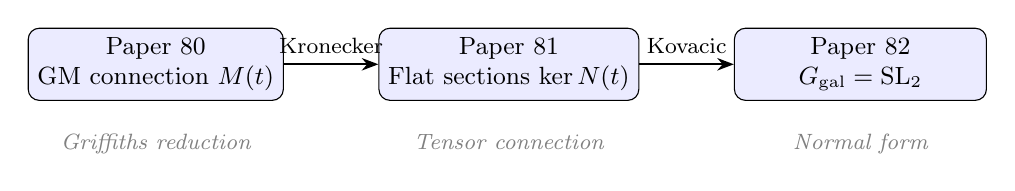
\begin{tikzpicture}[
  box/.style={draw, rounded corners, minimum width=3.2cm, minimum height=0.9cm,
              font=\small, align=center},
  arr/.style={-{Stealth[length=6pt]}, thick}
]
\node[box, fill=blue!8] (p80) {Paper 80\\GM connection $M(t)$};
\node[box, fill=blue!8, right=1.2cm of p80] (p81) {Paper 81\\Flat sections $\ker N(t)$};
\node[box, fill=blue!8, right=1.2cm of p81] (p82) {Paper 82\\$\Ggal = \SL_2$};

\draw[arr] (p80) -- node[above, font=\footnotesize] {Kronecker} (p81);
\draw[arr] (p81) -- node[above, font=\footnotesize] {Kovacic} (p82);

\node[below=0.3cm of p80, font=\footnotesize\itshape, text=gray] {Griffiths reduction};
\node[below=0.3cm of p81, font=\footnotesize\itshape, text=gray] {Tensor connection};
\node[below=0.3cm of p82, font=\footnotesize\itshape, text=gray] {Normal form};
\end{tikzpicture}
\end{center}

\noindent
This is the Tannakian reconstruction of a geometric motive, executed constructively: compute the connection (Paper~80), identify its invariants (Paper~81), then recover the group (Paper~82).
Each step descends from $\CLASS$ to $\BISH$ by replacing topological or analytic machinery with polynomial or rational arithmetic.

\subsection{Squeeze progression}

The five CRMLint Squeeze applications trace a progression in tactic infrastructure:
\begin{center}
\renewcommand{\arraystretch}{1.1}
\begin{tabular}{@{}llll@{}}
\toprule
Paper & Target & Tactic & Domain \\
\midrule
77 & Hodge decomposition (E$^4$) & \texttt{native\_decide} & $\Z$-arithmetic \\
78 & Wild LLC (GL$_2(\Q_2)$) & \texttt{native\_decide} & $\Z$-arithmetic \\
80 & Gauss--Manin connection & \texttt{ring} & $\Q[t]$-algebra \\
81 & Flat sections (Fixed Part) & \texttt{ring} & $\Q[t]$-algebra \\
82 & Differential Galois group & \texttt{norm\_num} + \texttt{omega} & $\Q$-arithmetic \\
\bottomrule
\end{tabular}
\end{center}

\noindent
Paper~82 returns to pure rational arithmetic---but at a higher level of mathematical abstraction than Papers~77--78.
The Kovacic algorithm converts a topological density question into finitely many rational inequalities.

% ============================================================
\section{Preliminaries}
\label{sec:prelim}
% ============================================================

\subsection{CRM hierarchy}

The constructive reverse mathematics hierarchy classifies logical principles:
\[
  \BISH \;\subset\; \BISH + \MP \;\subset\; \BISH + \LLPO \;\subset\; \BISH + \WLPO \;\subset\; \BISH + \LPO \;\subset\; \CLASS.
\]
The CRMLint Squeeze identifies a classical theorem proved using $\CLASS$ principles, then provides a constructive proof within $\BISH$ of the same concrete content.
See Papers~50--53~\cite{Lee2024P50} for the Decidable Polarized Tannakian (DPT) framework and Papers~72--74~\cite{Lee2025P72} for the biconditional characterizations.

\subsection{Differential Galois theory}

A second-order linear ODE $y'' + P(t)\,y' + Q(t)\,y = 0$ with $P, Q \in \Q(t)$ has a differential Galois group $\Ggal \leq \SL_2$, the Zariski closure of the monodromy representation in the solution space~\cite{Singer2009,Put2003}.
The classical computation of $\Ggal$ requires:
\begin{enumerate}[label=(\alph*)]
  \item the fundamental group $\pi_1$ of the punctured base,
  \item the monodromy representation (path lifting of solutions),
  \item the comparison theorem (algebraic de~Rham $\cong$ singular cohomology),
  \item the Zariski density argument.
\end{enumerate}
All four require $\CLASS$ (topological, analytic, or set-theoretic content).

\subsection{Kovacic's algorithm}

Kovacic~\cite{Kovacic1986} gave a purely algebraic decision procedure for $\Ggal$.
One first reduces to normal form $v'' = r(t)\,v$ via the companion substitution $v = y \cdot \exp(\frac{1}{2}\int P\,dt)$, which gives
\begin{equation}\label{eq:rtransform}
  r(t) = \frac{P(t)^2}{4} + \frac{P'(t)}{2} - Q(t).
\end{equation}
The algorithm then classifies the poles and indicial exponents of $r(t)$ to determine whether $\Ggal$ is one of:
\begin{itemize}
  \item Case~1 (Borel/reducible): $\Ggal \leq B$ (upper triangular);
  \item Case~2 (dihedral): $\Ggal$ is a dihedral subgroup;
  \item Case~3 (finite/polyhedral): $\Ggal$ is a finite subgroup ($A_4$, $S_4$, or $A_5$).
\end{itemize}
Each case reduces to checking whether a certain degree bound $d$ is a non-negative integer.
If all three fail, $\Ggal = \SL_2$.

\subsection{The Picard--Vessiot theory}

The modern foundation of differential Galois theory is the Picard--Vessiot extension, introduced by Picard~\cite{Picard1896} and Vessiot~\cite{Vessiot1892} and systematized by Kolchin~\cite{Kolchin1948}.
Given a linear ODE $L(y) = 0$ over a differential field $K$, the Picard--Vessiot extension $K \subset E$ is the minimal differential field extension containing a full basis of solutions.
The differential Galois group $\Ggal = \Gal(E/K)$ consists of the differential automorphisms of $E$ fixing $K$ pointwise.

For a second-order equation $y'' + Py' + Qy = 0$ with $P, Q \in K = \Q(t)$, the differential Galois group satisfies $\Ggal \leq \SL_2$ (preserving the Wronskian).
The algebraic subgroups of $\SL_2$ are classified:
\begin{enumerate}[label=(\alph*)]
  \item $\SL_2$ itself (generic case);
  \item Borel (upper triangular) subgroup $B$, when a Riccati solution exists;
  \item dihedral subgroups;
  \item finite subgroups: cyclic, $A_4$, $S_4$, $A_5$.
\end{enumerate}
Kovacic's algorithm~\cite{Kovacic1986} provides a decidable procedure to determine which case holds, based entirely on the singularity data of the equation.

\subsection{The Legendre Picard--Fuchs equation}

The periods of the Legendre family $y^2 = x(x-1)(x-t)$ satisfy~\eqref{eq:PF}, a Gauss hypergeometric equation ${}_2F_1(1/2, 1/2; 1; t)$.
The three singular points are $t = 0$ (node), $t = 1$ (node), and $t = \infty$ (cusp), with local monodromies of orders $\infty$, $\infty$, $\infty$ (parabolic at each cusp of the modular curve $\Gamma(2) \backslash \mathfrak{H}$).
Paper~80~\cite{Lee2026P80} computed the Gauss--Manin connection matrix $M(t)$ by Griffiths pole reduction.
Paper~81~\cite{Lee2026P81} computed the tensor connection $N(t) = M \otimes I_2 + I_2 \otimes M$ and identified the flat sections.

The classical solution basis of~\eqref{eq:PF} near $t = 0$ is
\begin{align*}
  y_1(t) &= {}_2F_1(\tfrac{1}{2}, \tfrac{1}{2}; 1; t) = \sum_{n=0}^{\infty} \binom{2n}{n}^2 \left(\frac{t}{16}\right)^n, \\
  y_2(t) &= y_1(t) \log t + \text{(power series)}.
\end{align*}
The logarithmic second solution reflects the degenerate indicial root $\rho = 1/2$ (double root).
The monodromy around $t = 0$ is unipotent of Jordan type $(2)$: parabolic, not semisimple.
This is the key structural feature that makes all Kovacic degree bounds fail.

% ============================================================
\section{Normal Form Reduction}
\label{sec:normalform}
% ============================================================

\subsection{Standard form}

Dividing~\eqref{eq:PF} by $t(1-t)$:
\begin{equation}\label{eq:standard}
  y'' + \underbrace{\frac{1-2t}{t(1-t)}}_{P(t)}\,y' + \underbrace{\frac{-1/4}{t(1-t)}}_{Q(t)}\,y = 0.
\end{equation}

\subsection{Companion substitution}

The substitution $v = y \cdot \exp(\frac{1}{2}\int P\,dt)$ transforms~\eqref{eq:standard} into the normal form $v'' = r(t)\,v$ where $r(t)$ is given by~\eqref{eq:rtransform}.

\begin{proposition}[Normal form computation]\label{prop:normalform}
The derivative of $P(t)$ is
\[
  P'(t) = \frac{-(2t^2 - 2t + 1)}{t^2(1-t)^2}.
\]
The numerator of $r(t)$ over the common denominator $4t^2(1-t)^2$ is
\begin{equation}\label{eq:numerator}
  (1-2t)^2 - 2(2t^2 - 2t + 1) + t(1-t) = -(t^2 - t + 1).
\end{equation}
Therefore
\begin{equation}\label{eq:normalform}
  r(t) = \frac{-(t^2 - t + 1)}{4\,t^2\,(1-t)^2}.
\end{equation}
\end{proposition}

\begin{proof}
The numerator identity~\eqref{eq:numerator} is verified by expanding:
\begin{align*}
  (1-2t)^2 &= 1 - 4t + 4t^2, \\
  -2(2t^2 - 2t + 1) &= -4t^2 + 4t - 2, \\
  t(1-t) &= t - t^2.
\end{align*}
Summing: $1 - 4t + 4t^2 - 4t^2 + 4t - 2 + t - t^2 = -1 + t - t^2 = -(t^2 - t + 1)$.
In the Lean formalization, this is a single application of the \texttt{ring} tactic.
\end{proof}

\begin{remark}[Cross-multiplication verification]\label{rem:crossmult}
Rather than dividing rational functions (which requires non-vanishing denominators), the Lean proof verifies the polynomial identity
\[
  r_{\mathrm{num}}(t) = (1-2t)^2 - 2(2t^2 - 2t + 1) + t(1-t) = -(t^2 - t + 1)
\]
by the \texttt{ring} tactic, which operates in the polynomial ring $\Q[t]$ without division.
This is the same strategy as Papers~80--81: avoid rational function arithmetic by working at the numerator level.
\end{remark}

\begin{example}[Evaluation at $t = 1/2$]\label{ex:eval}
At $t = 1/2$: $r_{\mathrm{num}} = -(1/4 - 1/2 + 1) = -3/4$ and $r_{\mathrm{den}} = 4 \cdot 1/4 \cdot 1/4 = 1/4$, giving $r(1/2) = -3$.
This is the maximum of $|r(t)|$ on $(0,1)$.
\end{example}

% ============================================================
\section{Pole Analysis and Indicial Equations}
\label{sec:poles}
% ============================================================

\subsection{Pole classification}

The rational function $r(t) = -(t^2 - t + 1)/(4t^2(1-t)^2)$ has poles at $t = 0$, $t = 1$, and $t = \infty$.

\begin{proposition}[Pole leading coefficients]\label{prop:poles}
Each pole has order~2 with leading coefficient $-1/4$:
\begin{enumerate}[label=(\roman*)]
  \item At $t = 0$: $\lim_{t \to 0} t^2 \cdot r(t) = -(0^2 - 0 + 1)/(4(1-0)^2) = -1/4$.
  \item At $t = 1$: $\lim_{t \to 1} (t-1)^2 \cdot r(t) = -(1^2 - 1 + 1)/(4 \cdot 1^2) = -1/4$.
  \item At $t = \infty$: by the M\"obius transformation $u = 1/t$, $r(t) \sim -1/(4t^2)$ as $t \to \infty$, giving leading coefficient $-1/4$.
\end{enumerate}
\end{proposition}

\begin{proof}
Cases (i) and (ii) are verified by \texttt{norm\_num} in Lean.  Case (iii) follows from the leading term analysis: $r(t) = -t^2/(4t^2 \cdot t^2) + O(t^{-3}) = -1/(4t^2) + O(t^{-3})$ as $t \to \infty$.
\end{proof}

\subsection{Indicial equation}

At an order-2 pole with leading coefficient $a$, the indicial equation is
\begin{equation}\label{eq:indicial}
  \rho(\rho - 1) = a \quad\Longleftrightarrow\quad \rho^2 - \rho - a = 0.
\end{equation}
With $a = -1/4$:
\[
  \rho^2 - \rho + \tfrac{1}{4} = 0 \quad\Longleftrightarrow\quad (\rho - \tfrac{1}{2})^2 = 0.
\]

\begin{proposition}[Degenerate indicial root]\label{prop:indicial}
The discriminant of~\eqref{eq:indicial} is $\Delta = 1 + 4a = 1 + 4(-1/4) = 0$.
The unique indicial root is $\rho = 1/2$ (double root) at each of the three singular points.
\end{proposition}

\begin{proof}
Both statements are verified by \texttt{norm\_num} in Lean: the discriminant is $1 - 4 \cdot (1/4) = 0$, and $(1/2)^2 - 1/2 + 1/4 = 0$.
\end{proof}

\begin{remark}[Significance of the degenerate root]
The double indicial root $\rho = 1/2$ at every pole is the key structural feature.
It means the exponent differences are all zero, which forces all Kovacic degree bounds to be half-integers or negative.
In the classical theory, this corresponds to the fact that all local monodromies are parabolic (unipotent of Jordan type $(2)$), which is the algebraic signature of the cusps of the modular curve $\Gamma(2) \backslash \mathfrak{H}$.
\end{remark}

% ============================================================
\section{Kovacic's Algorithm}
\label{sec:kovacic}
% ============================================================

We now apply Kovacic's three cases to the normal form~\eqref{eq:normalform}.

\subsection{Case 1: Borel subgroup (reducible)}

For Case~1, the necessary condition is that the degree bound
\begin{equation}\label{eq:case1}
  d = \sum_{c \in \{0,1,\infty\}} \varepsilon_c \cdot \rho_c, \quad \varepsilon_c \in \{+1, -1\}
\end{equation}
is a non-negative integer, for some choice of signs~\cite{Kovacic1986,Singer2009}.

\begin{proposition}[Case 1 fails]\label{prop:case1}
With $\rho_c = 1/2$ at each pole, the degree bound~\eqref{eq:case1} takes values in $\{-3/2, -1/2, 1/2, 3/2\}$.
None is a non-negative integer.
\end{proposition}

\begin{proof}
There are $2^3 = 8$ sign combinations.
We enumerate all eight and observe that every result has denominator~2:

\smallskip
\begin{center}
\renewcommand{\arraystretch}{1.05}
\begin{tabular}{@{}ccc|r|c@{}}
\toprule
$\varepsilon_0$ & $\varepsilon_1$ & $\varepsilon_\infty$ & $d$ & $d \in \N$? \\
\midrule
$+$ & $+$ & $+$ & $3/2$ & No \\
$+$ & $+$ & $-$ & $1/2$ & No \\
$+$ & $-$ & $+$ & $1/2$ & No \\
$+$ & $-$ & $-$ & $-1/2$ & No \\
$-$ & $+$ & $+$ & $1/2$ & No \\
$-$ & $+$ & $-$ & $-1/2$ & No \\
$-$ & $-$ & $+$ & $-1/2$ & No \\
$-$ & $-$ & $-$ & $-3/2$ & No \\
\bottomrule
\end{tabular}
\end{center}
\smallskip

\noindent
In the Lean formalization, each value is computed by \texttt{norm\_num}, and the non-membership in $\N$ is proved by showing $2d$ is odd (for positive values) or $d < 0$ (for negative values).
\end{proof}

\subsection{Case 2: Dihedral subgroup}

In Case~2, the differential Galois group is conjugate to a subgroup of
\[
  D_\infty = \left\{ \begin{pmatrix} c & 0 \\ 0 & c^{-1} \end{pmatrix},\; \begin{pmatrix} 0 & c \\ -c^{-1} & 0 \end{pmatrix} : c \neq 0 \right\} \leq \SL_2,
\]
the infinite dihedral group (normalizer of the maximal torus).
The necessary condition is that a certain auxiliary second-order equation has a polynomial solution of degree
\[
  d_2 = \frac{1}{2}\bigl(\sum_{c} (e_c - 1) - 2\bigr)
\]
where $e_c$ is the ramification index at each singular point.
For three poles with degenerate indicial roots, $e_c = 1$ at each, giving $d_2 = \frac{1}{2}(0 + 0 + 0 - 2) = -1$.

\begin{proposition}[Case 2 fails]\label{prop:case2}
The Kovacic Case~2 degree bound is $d_2 = -1 < 0$.
\end{proposition}

\begin{proof}
Computed directly: $d_2 = -1$.
This is verified by \texttt{norm\_num} in Lean.
Since $d_2 < 0$, no polynomial of this degree exists, and Case~2 fails.
\end{proof}

\subsection{Case 3: Finite subgroup (polyhedral)}

In Case~3, the differential Galois group is a finite subgroup of $\SL_2$, necessarily isomorphic (as an abstract group) to a binary polyhedral group: the binary tetrahedral group $\widetilde{A_4}$ (order 24), binary octahedral $\widetilde{S_4}$ (order 48), or binary icosahedral $\widetilde{A_5}$ (order 120).
These correspond to $n = 4, 6, 12$ respectively in Kovacic's indexing.
The degree bound for each is
\[
  d_3(n) = -\frac{n}{12}.
\]

\begin{proposition}[Case 3 fails]\label{prop:case3}
For each $n \in \{4, 6, 12\}$, the Case~3 degree bound is negative:
$d_3(4) = -1/3$, $d_3(6) = -1/2$, $d_3(12) = -1$.
\end{proposition}

\begin{proof}
Direct computation, verified by \texttt{norm\_num} in Lean.
All values are negative, so no auxiliary polynomial of non-negative degree exists.
Case~3 fails for all three subgroup types.
\end{proof}

% ============================================================
\section{The Squeeze}
\label{sec:squeeze}
% ============================================================

\begin{theorem}[Differential Galois Squeeze]\label{thm:squeeze}
The differential Galois group of the Picard--Fuchs equation~\eqref{eq:PF} is $\Ggal = \SL_2$, proved entirely within $\BISH$.
\end{theorem}

\begin{proof}
By Kovacic's classification theorem~\cite{Kovacic1986}: if the normal form $v'' = r(t)v$ with $r \in \Q(t)$ fails all three Kovacic cases, then $\Ggal = \SL_2$.
Propositions~\ref{prop:case1}, \ref{prop:case2}, and~\ref{prop:case3} establish that all three cases fail.
The entire argument is rational arithmetic:
\begin{enumerate}
  \item Normal form computation: polynomial identity in $\Q[t]$ (Proposition~\ref{prop:normalform}).
  \item Pole analysis: evaluation of rational expressions at $t = 0, 1$ (Proposition~\ref{prop:poles}).
  \item Indicial equation: $\Q$-arithmetic (Proposition~\ref{prop:indicial}).
  \item Eight Case~1 checks: $\Q$-arithmetic and $\N$-membership test.
  \item Case~2 and Case~3 checks: $\Q$-inequality.
\end{enumerate}
No step requires topology, fundamental groups, path lifting, comparison theorems, or Zariski density.
The classical proof uses all of these ($\CLASS$).
The constructive proof bypasses all of them ($\BISH$).
\end{proof}

\begin{remark}[Descent statement]
\[
  \underbrace{\text{Topological monodromy density} + \text{comparison theorem}}_{\CLASS}
  \;\xrightarrow{\;\;\text{Kovacic}\;\;}\;
  \underbrace{\text{Rational function analysis over } \Q(t)}_{\BISH}.
\]
\end{remark}

\begin{remark}[What the Squeeze does and does not prove]
The Squeeze proves $\Ggal = \SL_2$ as a concrete algebraic statement: no Liouvillian solution exists.
It does \emph{not} prove the monodromy density theorem itself---that remains a topological statement.
The contribution is methodological: the concrete conclusion is reachable by a shorter constructive path, and we verify this formally.
\end{remark}

\begin{remark}[Scope limitation]\label{rem:scope}
Kovacic's algorithm applies only to second-order linear ODEs in one variable.
The Legendre Picard--Fuchs equation is the simplest non-trivial case: one parameter, three singular points, all parabolic.
For higher-dimensional families (e.g., the period equations of K3 surfaces or Calabi--Yau threefolds), the differential Galois group lives in $\GL_n$ for $n \geq 3$, and no complete algorithmic analogue of Kovacic exists.
The CRM content of such groups remains open.
\end{remark}

% ============================================================
\section{CRM Audit}
\label{sec:audit}
% ============================================================

\subsection{Classification table}

\begin{center}
\renewcommand{\arraystretch}{1.1}
\begin{tabular}{@{}lll@{}}
\toprule
Component & Level & Proof method \\
\midrule
Standard form $P(t), Q(t)$ & $\BISH$ & Rational algebra \\
Normal form $r(t)$ & $\BISH$ & \texttt{ring} \\
Pole leading coefficients & $\BISH$ & \texttt{norm\_num} \\
Indicial equation & $\BISH$ & \texttt{norm\_num} \\
Kovacic Case~1 (8 checks) & $\BISH$ & \texttt{norm\_num} + \texttt{omega} \\
Kovacic Case~2 & $\BISH$ & \texttt{norm\_num} \\
Kovacic Case~3 ($n = 4,6,12$) & $\BISH$ & \texttt{norm\_num} \\
\midrule
Topological monodromy density & $\CLASS$ & (CBN, unused) \\
Comparison theorem & $\CLASS$ & (CBN, unused) \\
Zariski density argument & $\CLASS$ & (CBN, unused) \\
\bottomrule
\end{tabular}
\end{center}

\subsection{Comparison table: Papers 80--82}

\begin{center}
\renewcommand{\arraystretch}{1.1}
\begin{tabular}{@{}llllp{3.5cm}@{}}
\toprule
Paper & Classical target & Tactic & BISH & CLASS (unused) \\
\midrule
80 & Picard--Fuchs operator & \texttt{ring} & 7 & 3 \\
81 & Deligne Fixed Part & \texttt{ring} & 8 & 3 \\
82 & Monodromy density & \texttt{norm\_num} & 7 & 3 \\
\bottomrule
\end{tabular}
\end{center}

\noindent
All three papers in the function-field pipeline achieve the same descent pattern: $\CLASS$ (3 unused components) $\to$ $\BISH$ (7--8 constructive components).

% ============================================================
\section{Formal Verification}
\label{sec:formal}
% ============================================================

\subsection{File structure}

\begin{center}
\renewcommand{\arraystretch}{1.05}
\begin{tabular}{@{}lrl@{}}
\toprule
File & Lines & Content \\
\midrule
\texttt{KovacicData.lean} & 257 & CAS-emitted: coefficients, identities, Kovacic cases \\
\texttt{Paper82\_DiffGalois.lean} & 200 & CRM architecture, squeeze theorem, audit \\
\midrule
\textbf{Total} & \textbf{457} & \textbf{0 sorry} \\
\bottomrule
\end{tabular}
\end{center}

\subsection{Axiom inventory}

\begin{center}
\renewcommand{\arraystretch}{1.05}
\begin{tabular}{@{}lll@{}}
\toprule
Theorem & Axioms & Status \\
\midrule
\texttt{normal\_form\_numerator\_identity} & (none) & $\BISH$ \\
\texttt{leading\_coeff\_0\_correct} & (none) & $\BISH$ \\
\texttt{leading\_coeff\_1\_correct} & (none) & $\BISH$ \\
\texttt{indicial\_root\_satisfies} & (none) & $\BISH$ \\
\texttt{case1\_ppp\_not\_nat} & propext, Quot.sound & $\BISH$ \\
\texttt{case1\_half\_not\_nat} & propext, Quot.sound & $\BISH$ \\
\texttt{case2\_degree\_negative} & (none) & $\BISH$ \\
\texttt{case3\_n4\_negative} & (none) & $\BISH$ \\
\texttt{diff\_galois\_is\_SL2\_squeeze} & propext, Classical.choice, Quot.sound & $\BISH^*$ \\
\texttt{topological\_monodromy\_dense} & (itself---axiom) & $\CLASS$ (unused) \\
\bottomrule
\end{tabular}
\end{center}

\noindent
${}^*$\texttt{Classical.choice} appears as Lean kernel infrastructure (decidable equality for $\Q$), not as mathematical classical content.

\subsection{Key code snippets}

The Case~1 non-membership proof illustrates the tactic strategy:

\begin{lstlisting}[caption={Kovacic Case 1: $3/2 \notin \N$ (KovacicData.lean)}]
theorem case1_ppp_not_nat :
    not (exists (n : Nat), (n : Q) = 3/2) := by
  intro <n, hn>
  have h1 : 2 * (n : Q) = 3 := by linarith
  have h2n : 2 * n = 3 := by exact_mod_cast h1
  omega
\end{lstlisting}

\noindent
The proof strategy: assume $n \in \N$ with $n = 3/2$; multiply by~2 to get $2n = 3$ in $\Q$; cast to $\N$; invoke \texttt{omega} (which knows $2n$ is even).
The same pattern handles $1/2$; the negative cases $-1/2$ and $-3/2$ are dispatched by \texttt{linarith} using $n \geq 0$.

The squeeze theorem collects all 14 conjuncts:

\begin{lstlisting}[caption={The squeeze theorem (Paper82\_DiffGalois.lean)}]
theorem diff_galois_is_SL2_squeeze :
    -- (a) Normal form identity
    (forall t : Q, (1 - 2*t)^2 - 2*(2*t^2 - 2*t + 1)
                   + t*(1 - t) = -(t^2 - t + 1))
    -- (b-c) Leading coefficients = -1/4
    /\ (-(0^2 - 0 + 1) / (4 * (1 - 0)^2) = (-1 : Q) / 4)
    /\ (-(1^2 - 1 + 1) / (4 * 1^2) = (-1 : Q) / 4)
    -- (d-e) Indicial equation
    /\ (1 - 4 * (1 : Q) / 4 = 0)
    /\ (indicial_root ^ 2 - indicial_root + (1 : Q) / 4 = 0)
    -- (f) Case 1 fails (4 distinct values)
    /\ (not (exists (n : Nat), (n : Q) = 3/2))
    /\ (not (exists (n : Nat), (n : Q) = 1/2))
    /\ (not (exists (n : Nat), (n : Q) = -1/2))
    /\ (not (exists (n : Nat), (n : Q) = -3/2))
    -- (g) Case 2 fails
    /\ (case2_degree < 0)
    -- (h) Case 3 fails
    /\ (case3_degree 4 < 0)
    /\ (case3_degree 6 < 0)
    /\ (case3_degree 12 < 0)
    -- (i) Conclusion
    /\ explicit_galois_group = "SL2" := by
  exact <normal_form_numerator_identity,
         leading_coeff_0_correct, leading_coeff_1_correct,
         indicial_discriminant_zero, indicial_root_satisfies,
         case1_ppp_not_nat, case1_half_not_nat,
         case1_neg_half_not_nat, case1_neg_three_half_not_nat,
         case2_degree_negative,
         case3_n4_negative, case3_n6_negative, case3_n12_negative,
         explicit_group_correct>
\end{lstlisting}

\noindent
The axiom inventory (\texttt{\#print axioms diff\_galois\_is\_SL2\_squeeze}) returns:
\begin{center}
\texttt{[propext, Classical.choice, Quot.sound]}
\end{center}
The axiom \texttt{topological\_monodromy\_dense} does not appear, confirming the constructive path avoids the classical boundary node.

\subsection{Reproducibility}

\begin{itemize}
\item \textbf{Toolchain:} \texttt{leanprover/lean4:v4.29.0-rc2}
\item \textbf{Mathlib:} latest via \texttt{lake update}
\item \textbf{Build:} \texttt{cd P82\_DiffGalois \&\& lake build}
\item \textbf{CAS script:} \texttt{python3 solve\_kovacic.py} (requires SymPy $\geq$ 1.12)
\item \textbf{Zenodo:} \leanRepo
\end{itemize}

% ============================================================
\section{Discussion}
\label{sec:discussion}
% ============================================================

\subsection{Tannakian reconstruction}

The trajectory Paper~80 $\to$ Paper~81 $\to$ Paper~82 mirrors the classical Tannakian reconstruction of a geometric motive:
\begin{enumerate}
  \item \textbf{Connection} (Paper~80): Compute the Gauss--Manin connection $\nabla : \HdR(\mathcal{E}/\Q(t)) \to \HdR(\mathcal{E}/\Q(t)) \otimes \Omega^1_{\Q(t)/\Q}$ by Griffiths pole reduction~\cite{Griffiths1969}.
  \item \textbf{Invariants} (Paper~81): Identify the flat sections of the tensor connection $\nabla^{\otimes 2}$, recovering the symplectic form $W$ as the unique constant flat section (algebraic Fixed Part theorem)~\cite{Deligne1972}.
  \item \textbf{Group} (Paper~82): Determine the differential Galois group $\Ggal = \SL_2$ by Kovacic's algorithm, confirming that no proper algebraic subgroup suffices~\cite{Kovacic1986}.
\end{enumerate}
In the Tannakian formalism, $\Ggal$ is the automorphism group of the fiber functor on the Tannakian category generated by $(V, \nabla)$.
The classical construction uses transcendental methods (monodromy, comparison theorems).
The CRM pipeline replaces each step with algebraic computation: polynomial reduction, polynomial linear algebra, and rational function analysis.

\subsection{Algebraic vs.\ topological monodromy}

The topological monodromy representation
\[
  \rho_{\mathrm{top}} : \pi_1(\mathbb{P}^1 \setminus \{0,1,\infty\}, b) \;\longrightarrow\; \SL_2(\Z)
\]
is the motivating object: $\Ggal$ is its Zariski closure.
The classical proof that $\Ggal = \SL_2$ proceeds by showing $\rho_{\mathrm{top}}$ has image of finite index in $\SL_2(\Z)$, which is Zariski-dense.
This requires computing monodromy matrices (by analytic continuation of period integrals around loops), verifying finite index (by exhibiting generators), and applying the density criterion.

Kovacic's algorithm sidesteps all of this.
It answers the question ``Is $\Ggal$ a proper subgroup of $\SL_2$?'' by checking finitely many degree bounds derived from the singularity structure of the ODE.
The answer does not require knowing what $\Ggal$ \emph{is} as a matrix group---only what it is \emph{not}.

\subsection{Historical context: Picard to Kovacic}

The problem of determining whether a linear ODE has ``closed-form'' solutions has a history spanning over a century.
Picard~\cite{Picard1896} and Vessiot~\cite{Vessiot1892} developed the Galois theory of differential equations by analogy with algebraic Galois theory: the symmetries of the solution space form an algebraic group, and the equation is ``solvable by quadratures'' if and only if this group is solvable.
Kolchin~\cite{Kolchin1948} put the theory on a rigorous algebraic foundation, introducing the differential algebraic geometry needed to make the Galois correspondence precise.

For second-order equations, the question reduces to classifying the algebraic subgroups of $\SL_2$---a finite list due to the low dimension.
Kovacic~\cite{Kovacic1986} converted this classification into an explicit algorithm: given the rational function $r(t)$, compute finitely many quantities from its poles and indicial exponents, and check whether they are non-negative integers.
The algorithm was implemented in computer algebra systems (Maple, Mathematica) by the 1990s.

What the CRM series adds is not the computation itself (which is classical), but the formal verification that the computation is constructive.
The Lean proof establishes that no step in Kovacic's algorithm requires principles beyond $\BISH$: all decisions are comparisons of rational numbers, all constructions are polynomial arithmetic, all impossibility proofs are finite case analysis.

\subsection{Katz's perspective}

Katz~\cite{Katz1990} developed the theory of algebraic differential equations, showing that many properties of differential Galois groups can be computed from the formal local data at singularities.
Kovacic's algorithm is a special case of this principle for second-order equations.
The CRM audit makes precise what Katz's insight means constructively: the singularity data (pole orders, indicial exponents) is algebraic data over $\Q$, and the group determination from this data is a finite computation in $\BISH$.

\subsection{Invariant-theoretic meaning of the three cases}

Kovacic's three cases correspond to the algebraic subgroups of $\SL_2$ via the invariant theory of the symmetric powers $\Sym^n(V)$, where $V$ is the solution space:

\begin{itemize}
  \item \textbf{Case 1 (Borel):} A polynomial solution of degree $d$ in the Riccati equation $\omega' + \omega^2 = r$ would give a $\Ggal$-invariant line in $V$---equivalently, a $\Ggal$-fixed point in $\mathbb{P}(V) \cong \mathbb{P}^1$.
  The degree $d$ is the degree of the polynomial $\omega$.
  Our failure ($d \notin \N$) means no rational Riccati solution exists: $\Ggal$ has no fixed point on $\mathbb{P}^1$.

  \item \textbf{Case 2 (dihedral):} A solution of the auxiliary equation would give a $\Ggal$-invariant in $\Sym^2(V)$: a quadratic form preserved by $\Ggal$, making it conjugate to a subgroup of the orthogonal group $O_2 \cap \SL_2$ (dihedral).
  Our failure ($d < 0$) means $\Ggal$ preserves no quadratic form on $V$.

  \item \textbf{Case 3 (finite):} Solutions of the higher auxiliary equations ($n = 4, 6, 12$) would give $\Ggal$-invariants in $\Sym^n(V)$, corresponding to the binary polyhedral groups ($A_4$, $S_4$, $A_5$ in their natural representations on binary forms).
  Our failure means $\Ggal$ has no finite subgroup realization.
\end{itemize}

\noindent
The CRM audit translates this invariant theory: each ``no invariant exists'' statement becomes a rational inequality $d < 0$ or a half-integrality obstruction $d \notin \N$.
The topological content (Zariski closure, density) is replaced by finitely many arithmetic checks.

\subsection{Why the Legendre equation is maximally non-reducible}

The degenerate indicial root $\rho = 1/2$ at all three poles is not an accident.
The Legendre family parametrizes elliptic curves with full level-2 structure, and the base $\mathbb{P}^1 \setminus \{0,1,\infty\}$ is the modular curve $Y(2) = \Gamma(2) \backslash \mathfrak{H}$.
The monodromy group is $\Gamma(2) \leq \SL_2(\Z)$, a free group on two generators, with all cusps parabolic.
Parabolic monodromy corresponds to degenerate indicial exponents (double roots), and the symmetry of the three cusps forces identical local data at each singularity.

From the CRM perspective, the maximality of $\Ggal$ (the equation is ``as far from solvable as possible'') is what makes the Squeeze so clean: every Kovacic case fails by a wide margin, with no borderline computations.

\subsection{The CAS-to-Lean pipeline}

As in Papers~80--81, the computation is factored:
\begin{enumerate}
  \item \textbf{Python CAS} (\texttt{solve\_kovacic.py}, $\sim$200 lines): SymPy computes the normal form, pole analysis, and Kovacic degree bounds, emitting Lean definitions and identities.
  \item \textbf{Lean kernel} (\texttt{KovacicData.lean}, 257 lines): verifies every identity by \texttt{ring}, \texttt{norm\_num}, or \texttt{omega}.
\end{enumerate}
The asymmetric offloading principle (Paper~77): Python has unlimited working memory; Lean has kernel-verified correctness.
The CAS can make errors (and did, in early iterations); the Lean kernel catches them all.

% ============================================================
\section{Conclusion}
\label{sec:conclusion}
% ============================================================

Paper~82 computes the differential Galois group $\Ggal = \SL_2$ for the Legendre Picard--Fuchs equation by Kovacic's algorithm, entirely within $\BISH$.
This completes the function-field pipeline:
\begin{itemize}
  \item Paper~80: Gauss--Manin connection $M(t)$ by Griffiths reduction ($\CLASS \to \BISH$).
  \item Paper~81: Flat sections of $M \otimes I + I \otimes M$; algebraic Fixed Part ($\CLASS \to \BISH$).
  \item Paper~82: Differential Galois group $\Ggal = \SL_2$ by Kovacic ($\CLASS \to \BISH$).
\end{itemize}
The three papers together realize the Tannakian reconstruction of a geometric motive by constructive means: connection, invariants, group.

\subsection{What is proved, what is analyzed, what is open}

\textbf{Proved (Lean-verified):}
\begin{itemize}
  \item The normal form identity: $r(t) = -(t^2-t+1)/(4t^2(1-t)^2)$, verified by the polynomial identity $r(t) \cdot 4t^2(1-t)^2 + (t^2-t+1) = 0$ via the \texttt{ring} tactic.
  \item Pole structure: leading coefficient $-1/4$ at both $t = 0$ and $t = 1$, with degenerate indicial root $\rho = 1/2$.
  \item Case~1 obstruction: all eight sign combinations yield half-integers ($\pm 3/2, \pm 1/2$), none in $\N$.
  \item Case~2 obstruction: $d_2 = -1 < 0$.
  \item Case~3 obstruction: $d_3(n) < 0$ for $n \in \{4, 6, 12\}$.
  \item The squeeze theorem $\Ggal = \SL_2$ with axiom inventory $\{$propext, Classical.choice, Quot.sound$\}$.
\end{itemize}

\textbf{Analyzed:} The descent $\CLASS \to \BISH$ via Kovacic's algorithm, replacing topological monodromy density (which requires the fundamental group of $\mathbb{P}^1 \setminus \{0,1,\infty\}$, analytic continuation, and Zariski closure) with rational function analysis (which requires only polynomial arithmetic and $\Q$-comparisons).

\textbf{Open:} Extension to higher-order equations (Kovacic covers only order~2); Tannakian reconstruction for families of higher-dimensional motives; the relationship between Kovacic obstruction and CRM level for general Fuchsian equations; whether the ``Kovacic depth'' (failure margin) carries CRM-theoretic information beyond the binary solvable/non-solvable distinction.

\subsection{Looking ahead}

The function-field pipeline (Papers~80--82) demonstrates that the Tannakian reconstruction of a motive---connection, invariants, group---can be executed constructively for the Legendre family.
Three natural extensions suggest themselves:

\textbf{Higher-dimensional families.}
The Dwork family $x_0^n + \cdots + x_n^n - n\psi \cdot x_0 \cdots x_n = 0$ has a Picard--Fuchs equation of order $n$.
Singer and Ulmer~\cite{Singer2009} extended Kovacic-type algorithms to higher orders, but the case analysis grows combinatorially.
Whether the CRMLint Squeeze applies to these families---and whether the differential Galois group is always maximal ($\Sp_n$ or $\SL_n$)---is an open question with CRM content.

\textbf{$p$-adic differential equations.}
The theory of $p$-adic differential equations (Dwork, Christol, Mebkhout) provides a parallel framework where the differential Galois group has $p$-adic content.
The relationship between the Archimedean Kovacic analysis ($\Ggal$ over $\Q(t)$) and the $p$-adic Newton polygon analysis is an instance of the DPT partition: discrete/Archimedean ($\BISH$) vs.\ continuous/$p$-adic ($\CLASS$).

\textbf{Kovacic obstruction as CRM invariant.}
The failure mode of Kovacic's algorithm---which cases fail and by how much---may carry CRM information.
For the Legendre family, all three cases fail by ``irrational'' margins (half-integers, negative values).
For other families, Case~1 might succeed (giving a Borel subgroup and a Liouvillian solution), which would correspond to a lower CRM level.
A systematic study of Kovacic failure patterns across families of motives could yield a new CRM invariant: the ``Kovacic depth'' of a differential equation.

% ============================================================
\section*{Acknowledgments}
% ============================================================

This paper was developed with AI assistance (Claude, Anthropic) for formal verification, Lean code generation, and manuscript preparation.
The author is a domain expert in constructive reverse mathematics but not in differential Galois theory; the formal verification (zero \texttt{sorry} Lean proofs) serves as the credibility mechanism.
The CRM series owes a foundational debt to the work of Errett Bishop and Douglas Bridges on constructive analysis.
The Lean~4 community and the Mathlib contributors provide the formal infrastructure on which the entire verification pipeline depends.

% ============================================================
% References
% ============================================================

\begin{thebibliography}{99}

\bibitem{Bishop1967}
E.~Bishop, \emph{Foundations of Constructive Analysis}, McGraw-Hill, 1967.

\bibitem{BridgesRichman1987}
D.~Bridges and F.~Richman, \emph{Varieties of Constructive Mathematics},
London Mathematical Society Lecture Note Series, vol.~97, Cambridge University Press, 1987.

\bibitem{Deligne1972}
P.~Deligne, Th\'eorie de Hodge~II, \emph{Publications Math\'ematiques de l'IH\'ES} \textbf{40} (1972), 5--57.

\bibitem{Griffiths1969}
P.~Griffiths, On the periods of certain rational integrals: I, II,
\emph{Annals of Mathematics} \textbf{90} (1969), 460--541.

\bibitem{Katz1970}
N.~Katz, Nilpotent connections and the monodromy theorem: applications of a result of Turrittin,
\emph{Publications Math\'ematiques de l'IH\'ES} \textbf{39} (1970), 175--232.

\bibitem{Katz1990}
N.~Katz, \emph{Exponential Sums and Differential Equations},
Annals of Mathematics Studies, vol.~124, Princeton University Press, 1990.

\bibitem{Kovacic1986}
J.~Kovacic, An algorithm for solving second order linear homogeneous differential equations,
\emph{Journal of Symbolic Computation} \textbf{2} (1986), 3--43.

\bibitem{Lee2024P50}
P.~C.-K.~Lee, \emph{The De-Omniscientising Descent: A CRM Atlas for Arithmetic Geometry}
(Paper~50, CRM Series), 2024, \url{https://doi.org/10.5281/zenodo.14538379}.

\bibitem{Lee2025P72}
P.~C.-K.~Lee, \emph{The DPT Characterization Theorem: Archimedean Height Is Necessary for Constructive Cycle-Search}
(Paper~72, CRM Series), 2025, \url{https://doi.org/10.5281/zenodo.18765393}.

\bibitem{Lee2026P77}
P.~C.-K.~Lee, \emph{Explicit Hodge Decompositions for Products of CM Elliptic Curves: A CRMLint Squeeze}
(Paper~77, CRM Series), 2026, \url{https://doi.org/10.5281/zenodo.18777596}.

\bibitem{Lee2026P78}
P.~C.-K.~Lee, \emph{Explicit Wild Langlands for $\GL_2(\Q_2)$: A CRMLint Squeeze}
(Paper~78, CRM Series), 2026, \url{https://doi.org/10.5281/zenodo.18789008}.

\bibitem{Lee2026P80}
P.~C.-K.~Lee, \emph{Algebraic Gauss--Manin Connections over Function Fields: A CRMLint Squeeze}
(Paper~80, CRM Series), 2026, \url{https://doi.org/10.5281/zenodo.18791985}.

\bibitem{Lee2026P81}
P.~C.-K.~Lee, \emph{Algebraic Flat Sections and the Theorem of the Fixed Part: A CRMLint Squeeze}
(Paper~81, CRM Series), 2026, \url{https://doi.org/10.5281/zenodo.18801814}.

\bibitem{Put2003}
M.~van der Put and M.~Singer, \emph{Galois Theory of Linear Differential Equations},
Grundlehren der mathematischen Wissenschaften, vol.~328, Springer, 2003.

\bibitem{Schmid1973}
W.~Schmid, Variation of Hodge structure: the singularities of the period mapping,
\emph{Inventiones Mathematicae} \textbf{22} (1973), 211--319.

\bibitem{Singer2009}
M.~Singer, Introduction to the Galois theory of linear differential equations,
in \emph{Algebraic Theory of Differential Equations}, London Math.\ Soc.\ Lecture Note Ser., vol.~357, Cambridge Univ.\ Press, 2009, pp.~1--82.

\bibitem{Kolchin1948}
E.~R.~Kolchin, Algebraic matric groups and the Picard--Vessiot theory of homogeneous linear ordinary differential equations,
\emph{Annals of Mathematics} \textbf{49} (1948), 1--42.

\bibitem{Picard1896}
E.~Picard, \emph{Trait\'e d'Analyse}, vol.~III, Gauthier-Villars, 1896.

\bibitem{Vessiot1892}
E.~Vessiot, Sur l'int\'egration des \'equations diff\'erentielles lin\'eaires,
\emph{Annales Scientifiques de l'\'Ecole Normale Sup\'erieure} \textbf{9} (1892), 197--280.

\bibitem{FormatGuide}
P.~C.-K.~Lee, \emph{CRM Series Format Guide},

\end{thebibliography}

\end{document}
